% This file was created with tikzplotlib v0.9.17.
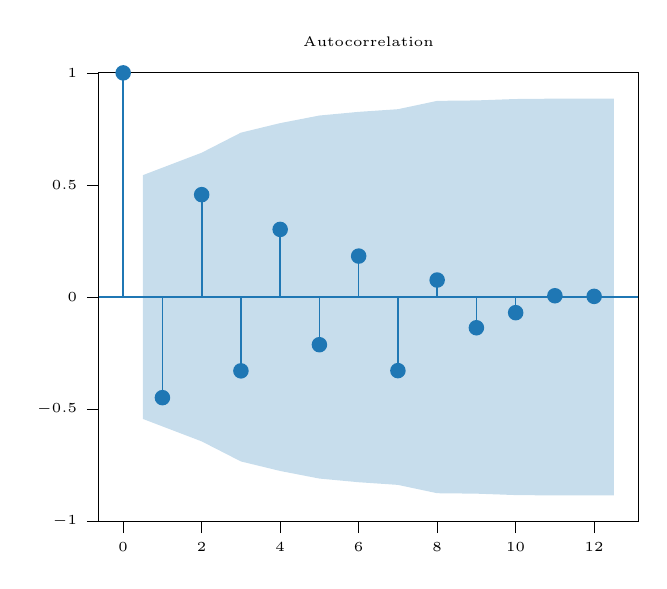
\begin{tikzpicture}

\definecolor{color0}{rgb}{0.12156862745098,0.466666666666667,0.705882352941177}

\begin{axis}[
font={\fontsize{3}{12}\selectfont},
tick align=outside,
tick pos=left,
title={Autocorrelation},
x grid style={white!69.0196078431373!black},
xmin=-0.625, xmax=13.125,
xtick style={color=black},
y grid style={white!69.0196078431373!black},
ymin=-1, ymax=1,
ytick style={color=black}
]
\path [fill=color0, fill opacity=0.25]
(axis cs:0.5,0.543596203409375)
--(axis cs:0.5,-0.543596203409375)
--(axis cs:2,-0.643849308609419)
--(axis cs:3,-0.733406245193091)
--(axis cs:4,-0.775866471522026)
--(axis cs:5,-0.809788174845269)
--(axis cs:6,-0.826124571613065)
--(axis cs:7,-0.837978779731899)
--(axis cs:8,-0.875162982581093)
--(axis cs:9,-0.877106743342688)
--(axis cs:10,-0.883410458607795)
--(axis cs:11,-0.885036031223623)
--(axis cs:12.5,-0.88504705505013)
--(axis cs:12.5,0.88504705505013)
--(axis cs:12.5,0.88504705505013)
--(axis cs:11,0.885036031223623)
--(axis cs:10,0.883410458607795)
--(axis cs:9,0.877106743342688)
--(axis cs:8,0.875162982581094)
--(axis cs:7,0.837978779731899)
--(axis cs:6,0.826124571613065)
--(axis cs:5,0.809788174845269)
--(axis cs:4,0.775866471522026)
--(axis cs:3,0.733406245193091)
--(axis cs:2,0.643849308609419)
--(axis cs:0.5,0.543596203409375)
--cycle;

\path [draw=color0, semithick]
(axis cs:0,0)
--(axis cs:0,1);

\path [draw=color0, semithick]
(axis cs:1,0)
--(axis cs:1,-0.448811885125943);

\path [draw=color0, semithick]
(axis cs:2,0)
--(axis cs:2,0.45684141522285);

\path [draw=color0, semithick]
(axis cs:3,0)
--(axis cs:3,-0.329293835289206);

\path [draw=color0, semithick]
(axis cs:4,0)
--(axis cs:4,0.301683609324544);

\path [draw=color0, semithick]
(axis cs:5,0)
--(axis cs:5,-0.212650687835832);

\path [draw=color0, semithick]
(axis cs:6,0)
--(axis cs:6,0.182698511379933);

\path [draw=color0, semithick]
(axis cs:7,0)
--(axis cs:7,-0.328310276009092);

\path [draw=color0, semithick]
(axis cs:8,0)
--(axis cs:8,0.0759155025892027);

\path [draw=color0, semithick]
(axis cs:9,0)
--(axis cs:9,-0.137033584416843);

\path [draw=color0, semithick]
(axis cs:10,0)
--(axis cs:10,-0.0697441420591051);

\path [draw=color0, semithick]
(axis cs:11,0)
--(axis cs:11,0.00574607907524478);

\path [draw=color0, semithick]
(axis cs:12,0)
--(axis cs:12,0.00295929314424705);

\addplot [semithick, color0]
table {%
-0.625 -2.22044604925031e-16
13.125 -2.22044604925031e-16
};
\addplot [semithick, color0, mark=*, mark size=2.5, mark options={solid}, only marks]
table {%
0 1
1 -0.448811885125943
2 0.45684141522285
3 -0.329293835289206
4 0.301683609324544
5 -0.212650687835832
6 0.182698511379933
7 -0.328310276009092
8 0.0759155025892027
9 -0.137033584416843
10 -0.0697441420591051
11 0.00574607907524478
12 0.00295929314424705
};
\end{axis}

\end{tikzpicture}
